\documentclass[12pt]{article}
\usepackage[margin=2cm, top = 2.5 cm]{geometry}
\usepackage{graphicx,tikz,tikz-network,tkz-euclide}
\usepackage{amsfonts,amsmath,amssymb}
\usepackage{tasks}
\usepackage{enumitem}
\usepackage{fancyhdr}
\usepackage{ifthen}
\usepackage{xparse}
\usepackage{tabularx}
\usepackage{cancel}
%\usepackage{tikz}
\usepackage{pgfplots}
\usetikzlibrary {positioning, calc}
\definecolor {processblue}{cmyk}{0.96,0,0,0}

\pgfplotsset{compat=1.5.1}

\title{Math Club Seventh Week Solutions}

\fancyhead[L]{Math Club W7 Solutions}
\fancyhead[R]{Nov 6, 2024}

\parindent 0pt
\date{November 2024}

\newcounter{problem}
\setcounter{problem}{0} % Initialize the counter at 0
\newcounter{sectionB}
\setcounter{sectionB}{0}

\newcommand{\problem}[2][]{
    \stepcounter{problem}%
    \noindent%
    \ifthenelse{\equal{\theproblem}{1}}{}{\\[1mm]}%
    \textbf{Problem $\mathbf{A\theproblem}$:}%
    \ifthenelse{\equal{#1}{}}{}{ (#1)}% Only include parentheses if (#1) if available
    \\[1mm] #2
    }

\newcommand{\problemB}[1]{
    \stepcounter{sectionB} % Increment the counter for Section B
    \noindent\textbf{Problem $\mathbf{B\thesectionB}$:} #1
    \\[1em] % Space after the problem statement
}

\newcommand{\multChoice}[5]{%
{\centering
\begin{tabular}{l @{\hskip 1.5cm} l @{\hskip 1.5cm} l @{\hskip 1.5cm} l @{\hskip 1.5cm} l}%
    A. #1 & B. #2 & C. #3 & D. #4 & E. #5
\end{tabular} \par}
}

\NewDocumentCommand{\multOpt}{O{3} m o o o o o o o}{%
    \ExplSyntaxOn
    \renewcommand{\arraystretch}{1}% Adjust spacing between rows if needed
    \begin{tabularx}{\textwidth}{@{}*{#1}{>{\centering\arraybackslash}X}@{}}%
        A. #2%
        \IfValueT{#3}{ & B. #3}%
        \IfValueT{#4}{ & C. #4}%
        \IfValueT{#5}{ & D. #5}%
        \IfValueT{#6}{ & E. #6}%
        \IfValueT{#7}{ & F. #7}%
        \IfValueT{#8}{ & G. #8}%
        \IfValueT{#9}{ & H. #9}%
  \end{tabularx}%
  \ExplSyntaxOff
}

\newcommand{\solution}[1]{
    \vspace{1em} % Add space before the solution
    \noindent\textbf{Solution:} #1
     % Add space after the solution
}

\setlength{\baselineskip}{5\baselineskip}

\usetikzlibrary {positioning}
%\usepackage {xcolor}
\definecolor {processblue}{cmyk}{0.96,0,0,0}
\newcommand{\myVertex}[3]{
    \Vertex[x=#1,y=#2,size=0.5,label=$#3$,position=90,fontscale=2,style={color=red}]{#3}
}
\newcommand{\simpleVertex}[3]{
    \Vertex[x=#1,y=#2,size=0.5,position=180,fontscale=2,style={color=red}]{#3}
}
\newcommand{\invisibleVertex}[3]{
    \Vertex[x=#1,y=#2,size=0.5,opacity =0,position=180,fontscale=2,style={color=white}]{#3}
}

\begin{document}
\sloppy
\thispagestyle{fancy}

\section*{AMATYC problems}

\begin{problem}[C][3][AMATYC Spring 2018/2]
   % Induction ^ Discrete ^ Student Math League
   Four rings of different sizes are stacked on a post, in ascending order (smallest on top). There are two other empty posts. You are able to move one ring at a time (taking the top ring from one post and moving it to another post), but you may never place a larger ring on a smaller ring. What is the minimum number of moves required to move the entire stack to the middle post?
   \vspace{-1em}
\begin{figure}[h]
  \centering
  \includegraphics[width=0.5\textwidth]{piles.png}
\end{figure}
\vskip -3mm
\end{problem}
\multOpt[5]{12}[14][15][16][17] 
\begin{solution}[C]
      Call $a_n$ the minimum number of moves required to move $n$ rings to some post, see that we can move the first $n-1$ rings in $a_{n-1}$ steps to the last post, then move the bigger ring to the middle post in one step and finally put all the $n-1$ rings back in another $a_{n-1}$ steps, so we must have $a_n=2a_{n-1}+1$, note that $a_1=1$, so
      \begin{align*}
         &a_2 = 2a_1+1=3\\
         &a_3 = 2a_2+1=7\\
         &a_4 = 2a_3+1=\boxed{15}
      \end{align*}
      The reader may check that $a_n=2^n-1$
\end{solution}

\begin{problem}[C][1][AMATYC Fall 2008/7]
   % Discrete ^ Student Math League
   The letters of $AMATYC$ are written as follows: Letters appear in increasing order of the number of line segments or arcs used to write them; identical letters do not appear consecutively. What is the required sequence?
\end{problem}

\begin{solution}
      $CT\!AY\!\!AM$
\end{solution}

\begin{problem}[P][2][AMATYC Spring 2008/7]
   % Probability ^ Student Math League
   A fair coin is labeled $A$ on one side and $M$ on the other; a fair die has two sides labeled $T$, two labeled $Y$, and two labeled $C$. The coin and die are each tossed three times. Find the probability that the six letters can be arranged to spell $AMATYC$.   
\end{problem}
\multOpt[5]{1/60}[1/48][1/36][1/24][1/12]
\begin{solution}[E]
   Let's focus on the coin first, we can rearrange $AMA$ in $3!/2!=3$ ways out of a total of $2^3=8$ possible outcomes, leaving probability $3/8$ to the coins. For the dice, see that we can rearrange $TYC$ in $3!=6$ ways of a total of $3^3=27$ possible outcomes, leaving probability $6/27=2/9$\\
    So our final answer should be $\frac{3}{8} \times \frac{2}{9} = \frac{1}{12}$
\end{solution}

\begin{problem}[A][5][AMATYC Spring 2001/12]
   % Algebra ^ Student Math League
   A set of 2001 different positive integers are arranged so that $a_1 < a_2 < a_3 < \dots < a_{2001}$. If the values with odd subscripts are all increased by 1, and those with even subscripts are all decreased by 1, which of the following must be true about the mean $\mu$ and median $m$ of the set?
    \begin{tasks}[label=\Alph*., label-width=13pt, before-skip=2mm, after-skip=0mm](2)
        \task $\mu$ decreases by less than 1 and $m$ decreases by 1
        \task $\mu$ increases by less than 1 and $m$ increases by 1
        \task $\mu$ decreases by less than 1 and $m$ is either unchanged or decreases by 1
        \task $\mu$ increases by less than 1 and $m$ is either unchanged or increases by 1
        \task $\mu$ and $m$ are both unchanged
    \end{tasks} 
\end{problem}

\begin{solution}[D]
   Call $S=a_1+a_2+\ldots+a_{2001}$, see that there are 1001 values with odd subscripts and 1000 values with even subscripts, so $S$ increases by 1 and $\mu$ increases by $1/2021<1$, also note that $m=a_{1001}$ at first, if $a_{1001}<a_{1002}-1$ then the median increases by 1, but if $a_{1001}=a_{1002}-1$ then now $m=a_{1002}$ which was the previous value of $a_{2001}$, so remains unchanged.
\end{solution}

\begin{problem}[A][4][AMATYC Fall 2021/4]
   % Trig ^ Algebra ^ Student Math League
   How many real ordered pairs $(x,y)$ with $|x| \leq 2$, $|y| \leq 2$ are solutions to the equation below?
   $$x^2 + 2x\sin(xy) + 1 = 0$$
\end{problem}
\multChoice{0}{1}{2}{3}{Infinitely many}

\begin{solution}[C]
   We know that, for real values $a,b,c$ and $a \neq 0$, the equation $ax^2+bx+c=0$ has real solutions for $x$ if and only if $b^2 \geq 4ac$, also that $1 \geq \sin x$:
    $$ 4 \geq 4\sin^2(xy) \geq 4$$
    That implies $\sin(xy)= \pm 1$ \\
    \begin{align*}
        x^2\pm2x+1=0 \\
        \iff x=\mp 1 \\
        \Rightarrow \sin(\mp y) = \pm1
    \end{align*}
    Since $|y| \leq 2$ we must have $y=\pm \frac{\pi}{2}$, that is, $(x,y)= (-1,\pi /2) , (1, -\pi/2)$.
\end{solution}

\begin{problem}[C][7][AMATYC Spring 2018/12]
   % Counting ^ Stars and Bars ^ Inclusion - Exlusion Principle ^ Student Math League
   A store carries 11 different types of bagels. Late one day, they had only 3 onion bagels left and 5 plain bagels left, but still had several dozen of each of the other types. If someone wanted to purchase a dozen bagels then, how many different combinations of 12 bagels would be possible (assuming that bagels of the same type are indistinguishable)? 
\end{problem}
\multOpt[5]{293,710}[594,880][594,946][646,184][646,646]
\begin{solution}[C]
   Call $x,y$ to the onion and plain bagels respectively, let $a_1,a_2,\ldots,a_9$ be the other types, we are asked count the different solution sets $(x,y,a_1,\ldots,a_9)$ of:
    $$ x+y+a_1+...+a_9 = 12$$
    Which is typically solved with the stars and bars method, if we fix $x+y=k$ then, we have a total of $\binom{12-k+8}{8} = \binom{20-k}{8}$
    By brute force we would have to consider all $4 \times 6$ pairs $(x,y)$, which can be done after some time with the help of some modular arithmetic to eliminate some possible solutions and let only $C$, instead we will use the inclusion-exclusion principle to adapt the restraints of $x$ and $y$.\medbreak
    Let $f(m,n)$ be the number of ordered pairs $(m,n,a_1,\ldots,a_9)$ of nonnegative integer solutions to our original equation, call $x_0=x-4$ , $y_0=y-6$, then our answer should be:
    \begin{align*}
        &f(x,y) - f(x_0,y) - f(x,y_0) + f(x_0,y_0) \\
        &= \binom{22}{12} - \binom{18}{8} - \binom{16}{6} + \binom{12}{2} \\
        &= \boxed{594,946}
    \end{align*}
    Note that the reasoning of this follows by starting from a total without any restrictions for the two bagels, then we remove the cases exceeding each of the limits, we add back again the cases in which both limits were exceeded simultaneously since we took them twice while subtracting. Without any restrictions we have $f(m,n) = \binom{12+11-1}{12}= \binom{22}{12}$, the reader may look at the stars and bars method to understand why
\end{solution}

\begin{problem}[P][7][AMATYC Fall 2021/19]
   % Counting ^ Probability ^ Student Math League
   Nine players are playing Texas Hold'em using a standard deck of 52 cards (2 10, J, Q, K, A in each of 4 suits). Each player is dealt two cards, and one player is dealt ``pocket kings" (two of the four kings in the deck). What is the probability (to the nearest \%) that another player is holding the only better hand, ``pocket aces"? \par
\end{problem}
\multOpt[5]{0\%}[1\%][2\%][3\%][4\%]
\begin{solution}[E]
   Let's remove the player who got the pocket kings from the game so that we have 8 players and 50 cards. We first want to know how many sets of 8 pairs could be drawn from the deck. The number of ways the first player could draw is given by $\binom{50}{2}$. Once these two cards are drawn, the next player has $\binom{48}{2}$ ways to draw. This continues for all 8 players, giving the total number of ways to draw 8 pairs as
    \begin{align} \setcounter{equation}{0}
        \frac{1}{8!}\binom{50}{2}\binom{48}{2}\dots\binom{38}{2}\binom{36}{2}
        =\frac{1}{8!}\cdot\frac{50!}{2!\,\bcancel{48!}}\cdot\frac{\bcancel{48!}}{2!\,\cancel{46!}}\dots\frac{\bcancel{38!}}{2!\,\cancel{36!}}\cdot\frac{\cancel{36!}}{2!\,34!}
        = \frac{50!}{2^8\,34!\,8!}
    \end{align}
    Note that we divided by 8! so that the order in which the cards were drawn didn't matter.\medbreak
    Now, say we have a game where a player draws the pocket aces. Note that this could happen $\binom{4}{2}=6$ ways (since there are 4 aces in the deck). Let's remove this player and the 2 aces they drew from the game, and consider the number of ways the other 7 pairs could be drawn from the remaining 48 cards. By a similar logic to before, this will work out to
    \begin{align}
        6\cdot\frac{1}{7!}\cdot\binom{48}{2}\binom{46}{2}\dots\binom{38}{2}\binom{36}{2}
        = \frac{6\cdot48!}{2^7\,34!\,7!}
    \end{align}
    Note that we multiplied by 6 to account for the different ways a pair of 2 aces could have been drawn. So (1) gives us the total number of possibilities, and (2) gives the number of successes. The probability of this event, then, is simply (2) over (1).
    \begin{align*}
        \frac{\left(\dfrac{6\cdot48!}{2^7\,34!\,7!}\right)}{\left(\dfrac{50!}{2^8\,34!\,8!}\right)} &= \frac{6\cdot48!}{2^7\,34!\,7!} \cdot \frac{2^8\,34!\,8!}{50!} \\
        &=\frac{6\cdot2\cdot8}{49\cdot50} \\[2mm]
        &\approx 0.039
    \end{align*}
    So after rounding, the probability works out to $\boxed{4\%}$.
\end{solution}

\begin{problem}[C][7][AMATYC Fall 2021/8]
   % Discrete ^ Student Math League
   In competitive soccer, a team that wins a match is awarded 3 points and the losing teams receive 0 points. In case of a draw (tie), both teams receive 1 point. A six team round robin (each team plays one match against each of the other five teams) is played, and Liverpool finishes with more points than any other team. What is the fewest number of points that Liverpool could have?
\end{problem}
\multOpt[5]{4}[5][6][7][8]
\begin{solution}[D]
   The total number of games played will be $\binom{6}{2}=15$. Since each team plays 5 games, 10 of these will be played without Liverpool. To get a plausible first guess, let's make the overall score as low as possible to allow Liverpool to win with a low score. Since ties result in a net score of 2 points ($+1$ to each team) whereas wins give 3 points total, we want to maximize the number of ties. \medbreak
        Imagine all of the first 14 games are a tie, and the last game results in a win for Liverpool. This gives us four teams with 5 points, one team with 4 points, and Liverpool with 7 points. So our tentative answer is 7. To determine if the score can drop to 6, let's consider how that would be accomplished. \medbreak
        First, we'll again minimize the score of the 10 non-Liverpool games by making them all ties for a net score of $10\cdot2=20$. Since only 5 other games can be played, the possibilities for Liverpool to win 6 points are (a) 2 wins, 3 losses or (b) 1 win, 1 loss, 3 ties. In case (a) the non-Liverpool teams score 9 points for a total of 29 points. And in case (b) the non-Liverpool teams score 6 points for a total of 26 points. In both cases, however, the score is higher than 25, meaning that at least one of Liverpool's five opponents matched or surpassed its score of 6. So 6 points does not work.\medbreak
        What about 5 or fewer points? Well, the minimum score for all games is $15\cdot2=30$ (15 ties). But if Liverpool earns 5 points and wins, no opponent could have earned more than 4 points. This gives a maximum score for this scenario of $5\cdot4+5=25$, which does not meet the minimum net score. Thus, Liverpool's minimum score is \fbox{7}.
\end{solution}


\begin{problem}[A][4][AMATYC Spring 2018/14]
   % Inequalities ^ Algebra ^ Student Math League
   $S$ is a set of four distinct real numbers, with greatest element $z$. If one adds each possible pair of elements of $S$, the results are (in ascending order): $\{2, 3, 4, 5, x, y\}$. Find the sum of all possible values of $z$.  
\end{problem}
\multOpt[5]{17/2}[26/3][9][28/3][10]
\begin{solution}[A]
   Let $S=\{a,b,c,z\}$ where $a<b<c<z$. The possible sums of element pairs are thus
    \[{\textstyle\sum} S=\{a+b,\ a+c,\ a+z,\ b+c,\ b+z,\ c+z\}\]
    We now wish to pair up these sums with the values $\{2, 3, 4, 5, x, y\}$. We can be sure that \[a+b\ <\ a+c\ <\ a+z \quad \text{and}\quad b+c\ <\ b+z\ <\ c+z\text{,}\]but we do not know whether $a+z$ or $b+c$ is bigger, so we must consider these possibilities seperately. Note, however, that in both cases
    \begin{align}
        a+b &= 2 \\
        a+c &= 3 \\
        \Rightarrow\ 2a+b+c &= 5
    \end{align}
    If $a+z > b+c$, then $a+z = 5$ and $b+c = 4$. Using (3), we find
    \begin{align*}
        2a+(4) = 5 \quad &\Rightarrow \quad a=\frac{1}{2} \\[2mm]
        \left(\frac{1}{2}\right) + z = 5 \quad &\Rightarrow \quad z=\frac{9}{2}
    \end{align*}
    Alternatively, if $a+z < b+c$, then $a+z = 4$ and $b+c = 5$. Using (3), we find
    \begin{align*}
        2a + (5) = 5 \quad &\Rightarrow \quad a=0 \\[2mm]
        (0) + z = 4 \quad &\Rightarrow \quad z=4
    \end{align*}
    And therefore the sum of possible values of $z$ is $\frac{9}{2} + 4 = \boxed{17/2}$.
\end{solution}

\begin{problem}[A][5][AMATYC Fall 2004/17]
   % MinMax ^ Student Math League
   If $x,y,z$ are positive integers with 
    $$x + 2y + 2z = 2005$$ 
    $$2x + 2y + z = 2004$$ 
    find the smallest possible value of $x + y + z$.
\end{problem}
\multOpt[5]{999}[1000][1001][1002][1003]
\begin{solution}[E]
   Call the top equation (1) and the bottom (2). We can eliminate a variable by subtracting (2) from (1) to get (3) $z = x+1$. We can then plug (3) into (1) to get
   \begin{align}\setcounter{equation}{3}
       x+2y+2(x+1)=2005 \iff 3x+2y = 2003
   \end{align}
   And what we are trying to find, then, is
   \begin{align*}
       \min(x+y+z) &= \min(2x+y+1)\notag\\
       &= \min(2x+y)+1
   \end{align*}
   To minimize $2x+y$, our goal is to make the $x$ as small as possible (since it is multiplied by 2) while still satisfying (4). If you plug $x=1$ (the smallest possible value of $x$) into (4), you will see that this works and gives $y=1000$. Thus,
   \begin{align*}
       \min(x+y+z) &= \min(2x+y)+1\\
       &=[2(1)+(1000)]+1 \\
       &=\boxed{1003}
   \end{align*}
   See that if you have any other solution $(x',y')$ where $x'>1$ , since $x'=2$ isn't a solution then $x' \geq 3$ , using (4):
   \begin{align*}
       y' &= \frac{2003}{2} - \frac{3}{2}x' \\
       2x'+ y' &= \frac{2003}{2} + \frac{x'}{2} \\
       &\geq \frac{2003+3}{2} = 1003
   \end{align*}
   Since any other solution is at least 1003, this is our minimum.
\end{solution}

\begin{problem}
   % Inequalities ^ Geometry ^ MinMax ^ Student Math League
   Circle $O$ has equation $x^2 + y^2 = 16$. If $P$ is $(1,0)$, $Q$ is $(-1,0)$, and $R$ is any point on circle $O$, what is the largest possible value of $\overline{PR} + \overline{QR}$?
\end{problem}
\multOpt[5]{8}[$2\sqrt{17}$][$6\sqrt{2}$][17/2][$4\sqrt{5}$]
\begin{solution}[B]
   For convenience, $a=\overline{PR}$ and $b=\overline{PR}$. We want $\max(a+b)$. Let's sketch the problem, labeling $P$, $Q$, $R$, and the origin $S$. This is depicted below on the left. \medbreak
    Observe that we've formed a triangle: $\triangle PQR$. If you draw $\overline{SR}$, you'll notice that this is a radius (with length 4) which divides $\triangle PQR$ into two smaller triangles ($\triangle QSR$ and $\triangle PSR$) and forms a pair of complementary angles ($\pi - \theta=\angle QSR$ and $\theta=\angle PSR$). This is depicted on the right.
    
    \begin{minipage}[t][][]{0.47\textwidth}\vspace{0pt}
        \begin{center}
        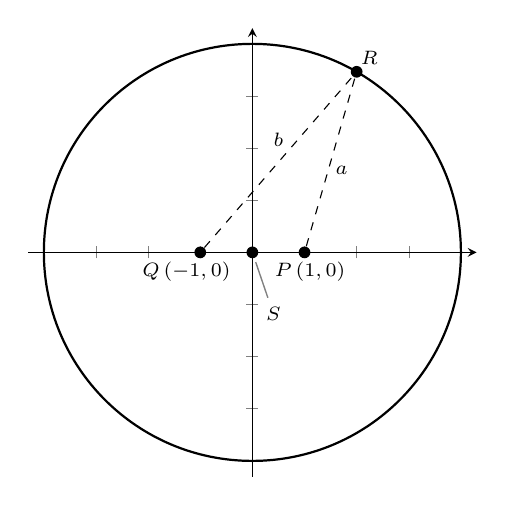
\begin{tikzpicture}[scale=1]
            \begin{axis} [
            axis lines = center,
            xmin = -4.3,
            xmax = 4.3,
            ymin = -4.3,
            ymax = 4.3,
            xtick = {-4,...,4},
            ytick = {-4,...,4},
            xticklabels = \empty,
            yticklabels = \empty,
            axis equal image,
            ]
            
            \draw[thick] (axis cs:0,0) circle [radius=4];
    
            \node[circle,fill,inner sep=1.5pt] (S) at (axis cs:0,0) {};
            %\node[anchor=north, fill=white, yshift=-2.5pt, inner sep=1.5pt] at (S) {\scriptsize$S$};
            \node[pin={[pin edge={line width = 0.5pt, color = gray}]275:\scriptsize$S$}] at (S) {};
    
            %\node[anchor=south east, xshift=1.5pt,yshift=-1pt] at (S) {\scriptsize$S$};
            
            \node[circle,fill,inner sep=1.5pt] (P) at (axis cs:1,0) {};
            \node[anchor=north, xshift=2pt] at (P) {\scriptsize$P\, (1,0)$};
            
            \node[circle,fill,inner sep=1.5pt] (Q) at (axis cs:-1,0) {};
            \node[anchor=north, xshift=-5pt] at (Q) {\scriptsize$Q\, (-1,0)$};
    
            \node[circle,fill,inner sep=1.5pt] (R) at (axis cs:2,3.464) {};
            \node[anchor=south west,xshift=-2pt,yshift=-1pt] at (R) {\scriptsize$R$};
    
            \draw[dashed, thin] (Q) -- (R) node[pos=0.5, above, yshift=2pt] {\scriptsize$b$};
    
            
            \draw[dashed, thin] (P) -- (R) node[pos=0.5, below, xshift=4pt, yshift=2pt] {\scriptsize$a$};
    
            \end{axis}
        \end{tikzpicture}
        \end{center}
    \end{minipage}\hfill%
    \begin{minipage}[t][][]{0.47\textwidth}
            \begin{center}
    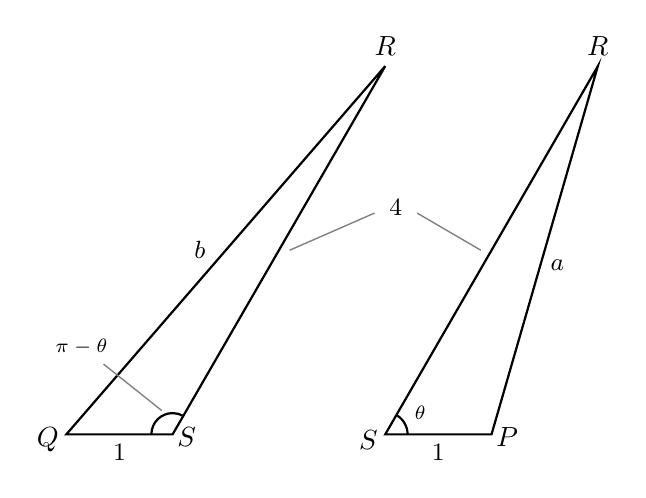
\begin{tikzpicture}[scale=1.35]

        \draw[thick] 
        (-2,0) coordinate (Q) node[anchor=east, xshift=1pt, yshift=-2pt] {$Q$} -- 
        (-1,0) coordinate (SL) node[anchor=north west, xshift=-2 pt, yshift=6pt] {$S$} -- 
        (1,3.464) coordinate (RL) node[anchor=south] {$R$} -- 
        cycle;

        \draw[thick] 
        (1,0) coordinate (SR) node[anchor=east, xshift=1pt, yshift=-2pt] {$S$} -- 
        (2,0) coordinate (P) node[anchor=north west, xshift=-2 pt, yshift=6pt] {$P$} -- 
        (3,3.464) coordinate (RR) node[anchor=south] {$R$} -- 
        cycle;

        \coordinate (ML) at ($(SL)!0.5!(RL) + (0.1,0)$);
        %\fill (ML) circle (2pt);
        \coordinate (MR) at ($(SR)!0.5!(RR) + (-0.1,0)$);
        %\fill (MR) circle (2pt);
        \coordinate (L) at ($(ML)!0.5!(MR) + (0.1,0.4)$);
        %\fill (L) circle (2pt);

        %side lengths
        \draw[color=gray, line width = 0.5pt] (ML) -- ($(L) + (-0.2,-0.05)$);
        \draw[color=gray, line width = 0.5pt] (MR) -- ($(L) + (0.2,-0.05)$);
        \node at (L) {\small$4$};
        \node[anchor=north] at ($(Q)!0.5!(SL)$) {\small$1$};
        \node[anchor=north] at ($(SR)!0.5!(P)$) {\small$1$};
        \node[anchor=east] at ($(Q)!0.5!(RL) + (-0.1,0)$) {\small$b$};
        \node[anchor=north] at ($(P)!0.5!(RR) + (0.12,0)$) {\small$a$};

        % left angle + label
        \draw[thick] ($(SL) + (-0.2,0)$) arc(0:-120:-0.2);
        \node[pin={[pin edge={line width = 0.5pt, color = gray}, pin distance=0.8cm]135:{\scriptsize$\pi-\theta$}}] at ($(SL)+(-0.01,0.15)$) {};
        \node at ($(SR)+(0.33,0.2)$) {\scriptsize$\theta$};
        \draw[thick] ($(SR) + (0.21,0)$) arc(0:60:0.21);
    \end{tikzpicture}\end{center}\end{minipage}\bigbreak

    Now, using law of cosines, observe that
    \begin{alignat}{2} \setcounter{equation}{0}
        a^2 &= 1^2 +4^2 -2(1)(4)\cos(\theta) &= 17 - 8\cos(\theta) \\
        b^2 &= 1^2 +4^2 -2(1)(4)\cos(\pi-\theta) \ &= 17 + 8\cos(\theta)
    \end{alignat}
    Also, as a consequence,%
    \begin{align}
        a &= \sqrt{17 - 8\cos(\theta)}\\
        b &= \sqrt{17 + 8\cos(\theta)}
    \end{align}
    Observe that adding (1) and (2) gives us $a^2+b^2=34$. Since we are looking for $a+b$, let's use \\ (3) and (4) to rewrite this as
    \begin{align*}
        a^2+b^2+2ab=34+2ab \quad \iff \quad (a+b)^2 &= 34+2ab\\
        &=34+2\sqrt{17^2 - 64\cos^2(\theta)}
    \end{align*}
    Since we know $\cos^2(\theta) \geq 0$ and $a,b > 0$, we can conclude
    \begin{align*}
        \max\left[(a+b)^2\right] &= 34+2\sqrt{17^2} = 68 \\
        \Rightarrow \max(a+b) &= \sqrt{68} = \boxed{2\sqrt{17}}
    \end{align*}
    Thus, $a+b$ is maximized when $\cos^2(\theta)$ is minimized, which occurs at $\theta = \pm\frac{\pi}{2}$. Returning to the sketches above, you would see that this is when $\triangle PQR$ is isosceles and points directly upwards or downwards, with $R=(0,\pm4)$.
\end{solution}

\begin{solution}[using Cauchy-Schwarz inequality]
   Let $R=(x,y)$, then $PR= \sqrt{(x-1)^2+y^2}$ and $\overline{PQ}=\sqrt{(x+1)^2+y^2}$, since R lies on the circle we must have $x^2+y^2=16$ , which further implies $PR^2+PQ^2=34$, then by making use of the Cauchy-Schwarz inequality:
    \begin{align*}
        (1+1)(PR^2 + PQ^2 ) &\geq (PR+PQ)^2 \\
        2\sqrt{17} = \sqrt{2 \times 34} &\geq (PR+PQ) 
    \end{align*}
    Note that we get the maximum when $PR=PQ \Rightarrow (x-1)^2=(x+1)^2 \Rightarrow x=0 \Rightarrow y^2=16$ , that is, when $R=(0,\pm4)$.
    
\end{solution}

%\section*{Calculus Problems} %in my opinion we should skip these since AMATYC is this week, what do you think
%yeah it's better to go just for AMATYC this time
\end{document}